\documentclass[a4paper]{article}

\usepackage[utf8]{inputenc}
\usepackage[T1]{fontenc}
\usepackage{graphicx}
\usepackage{fullpage}
\usepackage{hyperref}
\usepackage{caption}
\usepackage{subcaption}
\usepackage{float}
\floatstyle{boxed}
\restylefloat{figure}

\author{Titouan Christophe\\BA3 Computer Science ULB - 382957}
\date{\today}
\title{INFO-F-402 Project: Virtual Pet}

\begin{document}
\maketitle

\section{Scope}
A small virtual companion should be programmed in Scheme, and run on an ARM based Olimex LPC-2214H development board. Some electronic components could be connected to this board, such as leds, an LCD screen and an accelerometer. The final layout is presented on Figure \ref{fig:layout}. For each LED (program output, green, yellow or red), there's a corresponding button (user input). 

\begin{figure}[h]
  \centering
  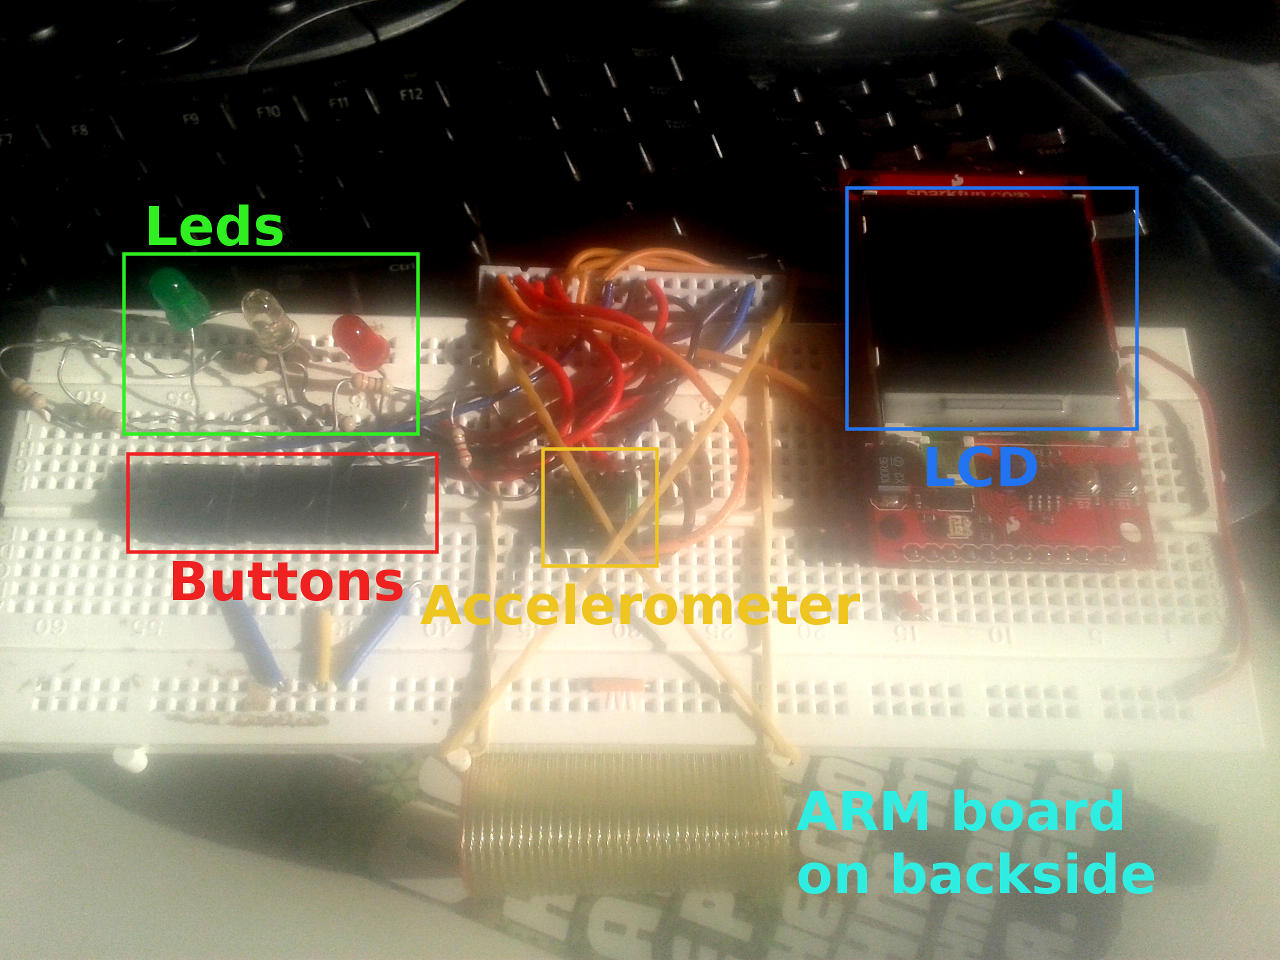
\includegraphics[width=0.5\textwidth]{Pictures/layout.png}
  \caption{\label{fig:layout} Overall layout of the electronic components}
\end{figure}

\subsection{Aptitudes (vital characteristics)}
The pet has 5 main continuous (floating value between 0 and 1) characteristics \textit{(happiness, submission, food, health and rest)}, which define its behaviour and likelihood to do or do not certain actions. There are also 2 discrete characteristics \textit{(poop count and toilet usage)} which act more as counters and impact the effects of the continous characteristics. They are described on Figure \ref{fig:aptitudes}. When the program starts, the continuous aptitudes are initialised to 0.75, while the discrete ones are initialised to zero.

\begin{figure}[h]
  \centering
  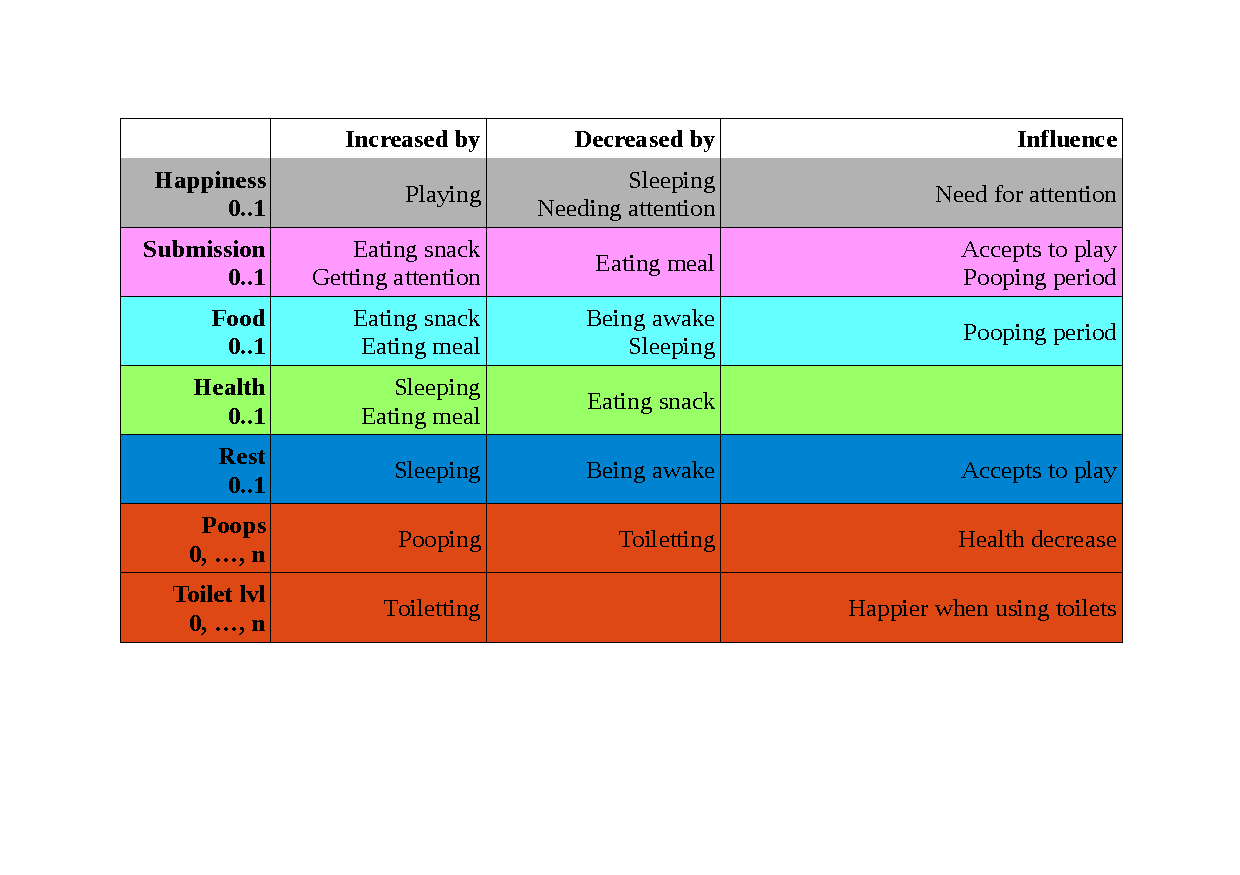
\includegraphics[width=\textwidth]{Aptitudes-balancing.pdf}
  \caption{\label{fig:aptitudes} Aptitudes with the colors used to represent them on LCD screen, and relation between each others}
\end{figure}

\section{Using the virtual pet}
\subsection{Main screen}
When the program starts, the LCD screen shows the actual state of the virtual pet. The characteristics are displayed in bars or as a smile (see Figure \ref{fig:smile}). If a characteristic is criticaly low ($ x < 0.125$), the bar background becomes red. The LEDs for buttons that could trigger an action are lit.

\subsection{Playing a game}
By pressing the green button, you enter a mini-game with the pet. This action is confirmed by a LED animation. When the animation has finished, the pet \textit{randomly}\footnote{The random generator is in fact the integer value returned by the accelerometer} choose a color, you have to press one of the 3 buttons in hope that it will be the one that the pet has chosen. If you find the right color first in a sufficiently short amount of time, the pet will be more happy. You exit the game mode when you pick the right color. Note that the pet won't accept to play if he is too tired or not submissive enough.

\subsection{Feeding the pet}
When pressing the yellow button, you can give some food to your pet. If you then click the green button, the pet will get a snack, with the red button it will receive a full meal. If  he eats a snack, it will be more happy (chocolate makes everyone happy\footnote{because it contains phenethylamine}), but its health will lower a bit (chocolate makes you fat). Also, it will be more submissive because he sees snacks as rewards. If he receives a full meal, it's health will increase a bit (vegetables are more than simply food: they contain vitamines, minerals, ...), but it will be a bit less submissive (unfortunately, he doesn't like vegetables). Once you have chosen some food, you'll have to wait a short time so that the pet can eat it.

\subsection{Pooping and toiletting}
From time to time, the pet will drop a poop on the bottom on the screen. If there are a lot of them, the pet's health is likely to decrease quicker. Also, the less the pet is submissive and the more he's fed, the more he will poop. To clean its droppings, click on the red button. Each time the pet clean his droppings, he gets more toilet trained. When he has a high toilet level, he gains some happiness each time he cleans his poops.

\subsection{Sleeping}
If the pet need some sleep, just flip him upside-down for a few seconds, then bring him back to a normal tilt. His eyes have now been replaced by an animated set of \textbf{Z}. Sleeping increases his rest, but slightly decreases his happiness and food fulfilling. To wake him up, simply do the same flip trick.

\subsection{Needing for attention}
When a vital characteristic (continous) reaches a critical point, or when the pet is awake and his owner didn't use it for a while, the virtual companion might ask for attention, by animating its leds repeatdly. To give him some attention, simply tilt him in any direction, or press a button.

\subsection{Death}
If any of the vitale characteristic (continous) reach zero, the pet dies. His screen becomes full of red, and the only way to resurect him is to press the reset button then relaunch the program. Obviously, all his characteristics will be reset (even the discretes ones).

\begin{figure}[h]
  \centering
  \begin{subfigure}[b]{0.3\textwidth}
    
\includegraphics[width=\textwidth]{Pictures/smiling.png}
    \caption{\label{fig:smile:happy} The pet is quite happy}
  \end{subfigure}
  \begin{subfigure}[b]{0.3\textwidth}
    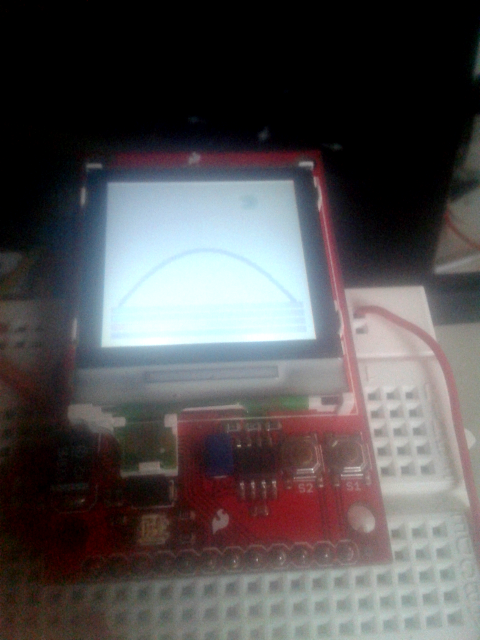
\includegraphics[width=\textwidth]{Pictures/unhappy.png}
    \caption{\label{fig:smile:unhappy} The pet is very unhappy}
  \end{subfigure}
  \begin{subfigure}[b]{0.3\textwidth}
    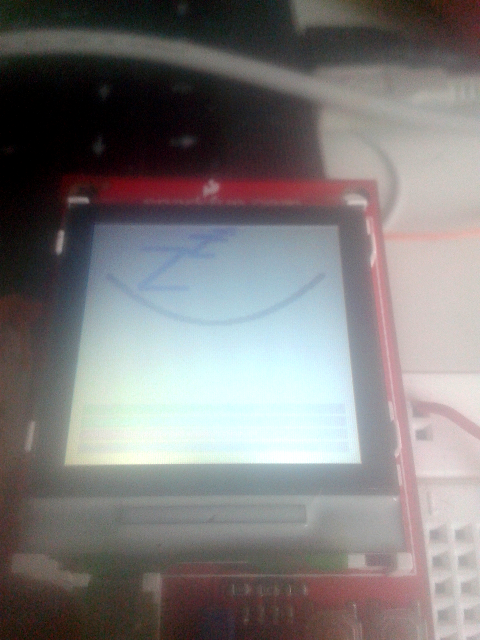
\includegraphics[width=\textwidth]{Pictures/sleeping.png}
    \caption{\label{fig:smile:sleeping} The pet is happy and sleeping}
  \end{subfigure}
  \caption{\label{fig:smile} Happiness representation as a smile. It is possible to see the other characteristics bars at the bottom of the screen, despite the bad photo quality.}
\end{figure}

\section{Implementation}
\subsection{Finite state machine}
As stated in the assignment, the virtual companion is implemented using a finite state machine. The framework given with the board examples\footnote{"state machine.scm" on \url{https://drive.google.com/folderview?id=0B3xYQ_2U35a8aUpmWklHZExBQlk}} was used. This library allows for the creation of states $\lambda$, which are functions responding to certain types of messages (kind of object-oriented programming). In particular, there are 3 interesting message types:

\paragraph{entry-action}
When received, call a no-arg function (a thunk) to initialize the state. Note that this function is decorated in this project to accomplish a few more tasks common to all states (update the LCD display and the last transition time for example; see also Section \ref{time})

\paragraph{exit-action}
When received, call a thunk to deinitialize the state, or updating global state variables (that is, the pet characteristics).

\paragraph{add-transition}
This method add a transition from this state. A transition defines a predicate $\lambda$ associated to a target state for a given type of message. Therefore, feeding a context message of this type will trigger the evaluation of the predicate $\lambda$. The target state becomes the current state if the predicate is true.

Figure \ref{fig:states} shows the overall finite state automaton map, where nodes are states and edges are transistions. As we can see, there is an entry state \texttt{Boot}, whose output function does all the hardware and global state variables initialisation. There is also a final state \texttt{Dead}. All the other states could be be entered and exited following the transitions rules. On the figure, there isn't enough space to fully describe each transition in details, however colors and (I hope to be) meaningful labels provide a general view of the pet's mind map.

\begin{figure}[h]
  \includegraphics[width=\textwidth]{states.eps}
  \caption{\label{fig:states} State machine graph}
\end{figure}

\subsection{Mainloop}
The main program is a tail-recursive function (therefore allowing for infinite recursion without stack growth) which feeds sensor informations, and a timing heartbeat to the state machine. Each sensor value is fed only if it differs from the value it had the last time it was fed. The heartbeat-triggered transitions are in pink on the FSM graph, those depending of accelerometer values are in cyan and the red, green and yellow edges stand for the color buttons. Black edges represent more complex predicates or a set of possible messages.

\subsection{Graphics}
The LCD screen merely implements a unique primitive: filling a rectangle from a point with a width and a height. You can see on program boot that the rectangle filling is quite slow, and the filling time depends of the rectangle size. Also, the function \texttt{fill-rectangle!} provided in the lib supporting the board blocks until the screen is totally up to date. 

The method used to draw more complex shapes, such as the pet's smile, his eyes, or the Zzz when he's sleeping is inspired by mathematical function plots. The smile is a parabola centered on the point $(x_0, y_0)$ of the screen, which is the set of points verifying the equation $y = y_0 + a(x - x_0)^2 $, where $a$ is the happinness factor. The eyes are constituted of 2 half circles that again could be written as functions of the center $(x_0, y_0)$ and a radius, or the Zzz that are made of lines.

Therefore all non-rectangular shapes are built from functions that returns a $\lambda(x) \rightarrow y$, which are used by a render function drawing a 3x3 square on screen for each $(x, y)$ pair. While the drawing of each square is fast because of the small filling area, the entire processing is relatively slow. I see two potential reasons for this: 
\begin{itemize}
  \item The constant time to send a single command to the screen, regardless the filling area, could not be reduced
  \item While the drawing algorithm itself is simple and straightforward, its Scheme implementation might be slow because resolving variable in highly nested lambdas could take a lot of time (because the interpreter might have to traverse a bunch of environment frames)
\end{itemize}

Making the graphical part faster would be a nice topic for this project continuation, however the moving graphics in construction, like some kind of animation, make this pet more appealing. For example the effect of the eyes gradually opening is totally unwanted but nice to see

\subsection{Time}
\label{time}
Since a lot of functionnality depends on time (characteristics evolution, needing for attention, ...), the timer of the microcontroller is used. It is initialised at boot time, to provide a duty cycle of 1 ms. When the FSM enters a new state, the current time is stored, and the helper function \texttt{state-uptime} could return the number of milliseconds since last state change. Also, two functions inspired by the Arduino platform were implemented, \texttt{millis}, which return the total uptime in ms (read timer), and \texttt{delayms} wich actively waits a given number of ms. 

\end{document}
